\documentclass[landscape]{slides}
\usepackage{url}
\usepackage{amsmath}
\usepackage{graphicx}
\usepackage{color}
\usepackage{epic,ecltree}
%\usepackage{bar}
\usepackage{eclbip}
\usepackage{multicol}
\usepackage{algorithmic}
\usepackage{algorithm}
\renewcommand{\algorithmicrequire}{\textbf{Input:}}
\renewcommand{\algorithmicensure}{\textbf{Output:}}
\renewcommand{\algorithmiccomment}[1]{// {\em #1}}

\definecolor{darkblue}{rgb}{0,0,0.8}
\definecolor{darkgreen}{rgb}{0,0.8,0}
\definecolor{purple}{rgb}{0.6,0,0.6}
\definecolor{red}{rgb}{1,0,0}

\newcommand{\example}[1]{\textcolor{darkblue}{\rm #1}}
\newcommand{\maths}[1]{\textcolor{purple}{#1}}
\newcommand{\reference}[1]{\vspace{-2mm}\begin{flushright}\textcolor{purple}{\tiny [from #1]}\end{flushright}\vspace{-7mm}}

\begin{document}
\title[Chapter 4: Word-Based Models]{Chapter 4\\[1cm] Word-based models}
\author[Philipp Koehn]{}
\date{Statistical Machine Translation}

\maketitle
%%%%%%%%%%%%%%%%%%%%%%%%%%%%%%%%%%%%%%%%%%%%%%%%%%%%%%%%%%%%%%%%%%%%%%%%%%%%

\slide{Lexical Translation}
\vspace{10mm}
\begin{itemize}
\item How to translate a word $\rightarrow$ look up in dictionary

\begin{quotation}
\example{{\bf Haus} --- house, building, home, household, shell.}
\end{quotation}

\item Multiple translations
\begin{itemize}
\item some more frequent than others
\item for instance: \example{house}, and \example{building} most common
\item special cases: \example{Haus} of a \example{snail} is its \example{shell}
\end{itemize}
\item Note: In all lectures, we translate from a foreign language into English
\end{itemize}

%%%%%%%%%%%%%%%%%%%%%%%%%%%%%%%%%%%%%%%%%%%%%%%%%%%%%%%%%%%%%%%%%%%%%%%%%%%%

\slide{Collect Statistics}
\vspace{20mm}
\begin{center}
Look at a parallel corpus (German text along with English translation)

\vspace{10mm}
\begin{tabular}{|l|r|r|} \hline
{\bf Translation of {\em Haus}} & {\bf Count} \\ \hline
\example{house}      & 8,000 \\ \hline
\example{building}   & 1,600 \\ \hline  
\example{home}       &  200 \\ \hline
\example{household}  &  150 \\ \hline
\example{shell}      &   50 \\ \hline
\end{tabular}
\end{center}


%%%%%%%%%%%%%%%%%%%%%%%%%%%%%%%%%%%%%%%%%%%%%%%%%%%%%%%%%%%%%%%%%%%%%%%%%%%%

\slide{Estimate Translation Probabilities}
\vspace{20mm}
\begin{center}
Maximum likelihood estimation
\vspace{5mm}
\begin{equation*}
p_f(e) = 
\begin{cases}
0.8 &   \text{if $e$ = \example{house}}, \\
0.16 &  \text{if $e$ = \example{building}}, \\
0.02 &  \text{if $e$ = \example{home}}, \\
0.015 & \text{if $e$ = \example{household}}, \\
0.005 & \text{if $e$ = \example{shell}}.
\end{cases}
\end{equation*}
\end{center}

%%%%%%%%%%%%%%%%%%%%%%%%%%%%%%%%%%%%%%%%%%%%%%%%%%%%%%%%%%%%%%%%%%%%%%%%%%%%

\slide{Alignment}
\begin{itemize}
\item In a parallel text (or when we translate), we align words in one language with the words in the other

\begin{center}
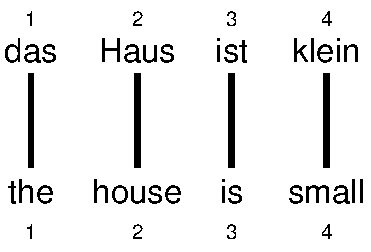
\includegraphics[scale=1.5]{haus-ist-klein-alignment.pdf}
\end{center}

\item Word positions are numbered 1--4
\end{itemize}

%%%%%%%%%%%%%%%%%%%%%%%%%%%%%%%%%%%%%%%%%%%%%%%%%%%%%%%%%%%%%%%%%%%%%%%%%%%%

\slide{Alignment Function}
\vspace{10mm}
\begin{itemize}
\item Formalizing alignment with an alignment function
\vspace{10mm}
\item Mapping an English target word at position \maths{$i$} to a German source word at position  \maths{$j$} with a function  \maths{$a: i \rightarrow j$}
\vspace{10mm}
\item Example
\maths{\begin{equation*} 
a: \{1 \rightarrow 1, 2 \rightarrow 2, 3 \rightarrow 3, 4 \rightarrow 4\}
\end{equation*}}
\end{itemize}

%%%%%%%%%%%%%%%%%%%%%%%%%%%%%%%%%%%%%%%%%%%%%%%%%%%%%%%%%%%%%%%%%%%%%%%%%%%%

\slide{Reordering}
\begin{center}\vspace{10mm}
Words may be reordered during translation\\[10mm]
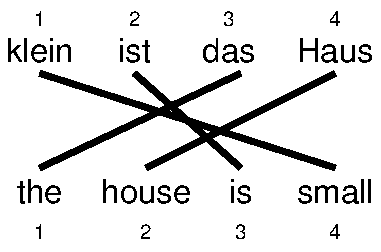
\includegraphics[scale=1.5]{haus-ist-klein-alignment-reordered.pdf}\\[10mm]
 \maths{$a: \{ 1 \rightarrow 3, 2 \rightarrow 4, 3 \rightarrow 2, 4 \rightarrow 1 \}$}
\end{center}

%%%%%%%%%%%%%%%%%%%%%%%%%%%%%%%%%%%%%%%%%%%%%%%%%%%%%%%%%%%%%%%%%%%%%%%%%%%%

\slide{One-to-Many Translation}
\begin{center}\vspace{10mm}
A source word may translate into multiple target words \\[10mm]
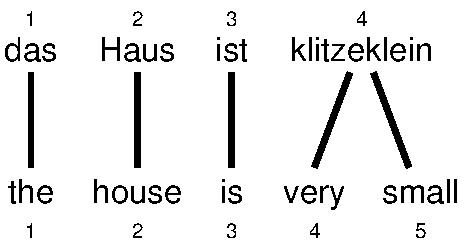
\includegraphics[scale=1.5]{haus-ist-klein-alignment-multiple.pdf}\\[10mm]
\maths{$a: \{ 1 \rightarrow 1, 2 \rightarrow 2, 3 \rightarrow 3, 4 \rightarrow 4, 5 \rightarrow 4 \}$}
\end{center}

%%%%%%%%%%%%%%%%%%%%%%%%%%%%%%%%%%%%%%%%%%%%%%%%%%%%%%%%%%%%%%%%%%%%%%%%%%%%

\slide{Dropping Words}
\begin{center}\vspace{7mm}
Words may be dropped when translated\\
(German article \example{das} is dropped)\\[10mm]
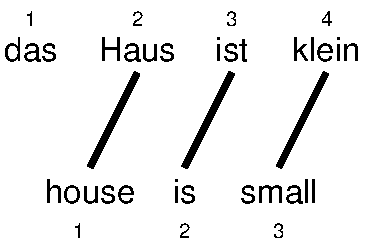
\includegraphics[scale=1.5]{haus-ist-klein-alignment-zerofert.pdf}\\[10mm]
\maths{$a: \{ 1 \rightarrow 2, 2 \rightarrow 3, 3 \rightarrow 4 \}$}
\end{center}

%%%%%%%%%%%%%%%%%%%%%%%%%%%%%%%%%%%%%%%%%%%%%%%%%%%%%%%%%%%%%%%%%%%%%%%%%%%%

\slide{Inserting Words}
\begin{itemize}
\item Words may be added during translation
\begin{itemize}
\item The English \example{just} does not have an equivalent in German
\item We still need to map it to something: special {\sc null} token
\end{itemize}
\begin{center}
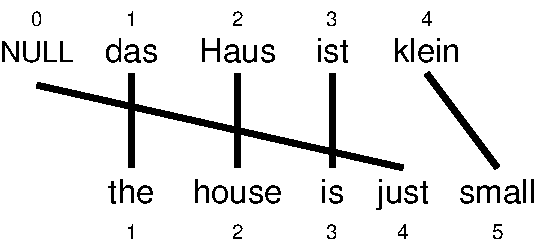
\includegraphics[scale=1.5]{haus-ist-klein-alignment-nullgen.pdf}\\[10mm]
\maths{$a: \{ 1 \rightarrow 1, 2 \rightarrow 2, 3 \rightarrow 3, 4 \rightarrow 0, 5 \rightarrow 4 \} $}
\end{center}
\end{itemize}

%%%%%%%%%%%%%%%%%%%%%%%%%%%%%%%%%%%%%%%%%%%%%%%%%%%%%%%%%%%%%%%%%%%%%%%%%%%%

\slide{IBM Model 1}
\begin{itemize}
\item Generative model: break up translation process into smaller steps
\begin{itemize} \vspace{-3mm}
\item IBM Model 1 only uses lexical translation
\end{itemize} 
\item Translation probability 
\begin{itemize} \vspace{-3mm}
\item for a foreign sentence \maths{{\bf f} $= (f_1, ..., f_{l_f})$} of length  \maths{$l_f$}
\item to an English sentence  \maths{{\bf e} $= (e_1, ..., e_{l_e})$} of length  \maths{$l_e$} 
\item with an alignment of each English word  \maths{$e_j$} to a foreign word  \maths{$f_i$} according to the alignment function  \maths{$a: j \rightarrow i$}
 \maths{\begin{equation*}
p({\bf e},a|{\bf f}) = 
\frac{\epsilon}{(l_f+1)^{l_e}} \prod_{j=1}^{l_e} t(e_j|f_{a(j)})
\end{equation*}}
\item parameter  \maths{$\epsilon$} is a normalization constant
\end{itemize}
\end{itemize}

%%%%%%%%%%%%%%%%%%%%%%%%%%%%%%%%%%%%%%%%%%%%%%%%%%%%%%%%%%%%%%%%%%%%%%%%%%%%

\slide{Example}
\vspace{10mm}
\begin{tabular}{cccc} 
\example{das} & \example{Haus} & \example{ist} & \example{klein} \\

\begin{tabular}{|l|l|} \hline
\maths{$e$} & \maths{$t(e|f)$} \\ \hline
\example{the} & 0.7 \\ \hline
\example{that} & 0.15 \\ \hline
\example{which} & 0.075 \\ \hline
\example{who} & 0.05 \\ \hline
\example{this} & 0.025 \\ \hline
\end{tabular}

&

\begin{tabular}{|l|l|} \hline
\maths{$e$} & \maths{$t(e|f)$} \\ \hline
\example{house}     & 0.8 \\ \hline
\example{building}  & 0.16 \\ \hline
\example{home}      & 0.02 \\ \hline
\example{household} & 0.015 \\ \hline
\example{shell}     & 0.005 \\ \hline
\end{tabular}

&

\begin{tabular}{|l|l|} \hline
\maths{$e$} & \maths{$t(e|f)$} \\ \hline
\example{is}      & 0.8 \\ \hline
\example{'s}      & 0.16 \\ \hline
\example{exists}  & 0.02 \\ \hline
\example{has}     & 0.015 \\ \hline
\example{are}     & 0.005 \\ \hline
\end{tabular}

&

\begin{tabular}{|l|l|} \hline
\maths{$e$}& \maths{$t(e|f)$} \\ \hline
\example{small} & 0.4 \\ \hline
\example{little} & 0.4 \\ \hline
\example{short} & 0.1 \\ \hline
\example{minor} & 0.06 \\ \hline
\example{petty} & 0.04 \\ \hline
\end{tabular}
\end{tabular}

\maths{\begin{equation*}
\begin{split}
p(e,a|f) &= \frac{\epsilon}{4^3} 
\times t(\mbox{\example{the}}|\mbox{\example{das}}) 
\times t(\mbox{\example{house}}|\mbox{\example{Haus}}) 
\times t(\mbox{i\example{s}}|\mbox{\example{ist}}) 
\times t(\mbox{\example{small}}|\mbox{\example{klein}}) 
\\
&= \frac{\epsilon}{4^3} 
\times 0.7 \times 0.8 \times 0.8 \times 0.4 \\
&= 0.0028 \epsilon\\
\end{split}
\end{equation*}}

%%%%%%%%%%%%%%%%%%%%%%%%%%%%%%%%%%%%%%%%%%%%%%%%%%%%%%%%%%%%%%%%%%%%%%%%%%%%

\slide{Learning Lexical Translation Models}
\vspace{10mm}
\begin{itemize}
\item We would like to estimate the lexical translation probabilities \maths{$t(e|f)$} from a parallel corpus
\item ... but we do not have the alignments
\item Chicken and egg problem
\begin{itemize}
\item if we had the {\em alignments},\\ $\rightarrow$ we could estimate the {\em parameters} of our generative model\\[-3mm]
\item if we had the {\em parameters},\\ $\rightarrow$ we could estimate the {\em alignments}
\end{itemize}
\end{itemize}

%%%%%%%%%%%%%%%%%%%%%%%%%%%%%%%%%%%%%%%%%%%%%%%%%%%%%%%%%%%%%%%%%%%%%%%%%%%%

\slide{EM Algorithm}
\vspace{20mm}
\begin{itemize}
\item Incomplete data
\begin{itemize}
\item if we had {\em complete data}, would could estimate {\em model}
\item if we had {\em model}, we could fill in the {\em gaps in the data}
\end{itemize}
\item Expectation Maximization (EM) in a nutshell
\begin{enumerate}
\item initialize model parameters (e.g. uniform)
\item assign probabilities to the missing data
\item estimate model parameters from completed data
\item iterate steps 2--3 until convergence 
\end{enumerate}
\end{itemize}


%%%%%%%%%%%%%%%%%%%%%%%%%%%%%%%%%%%%%%%%%%%%%%%%%%%%%%%%%%%%%%%%%%%%%%%%%%%%

\slide{EM Algorithm}
\vspace{10mm}
\begin{center}
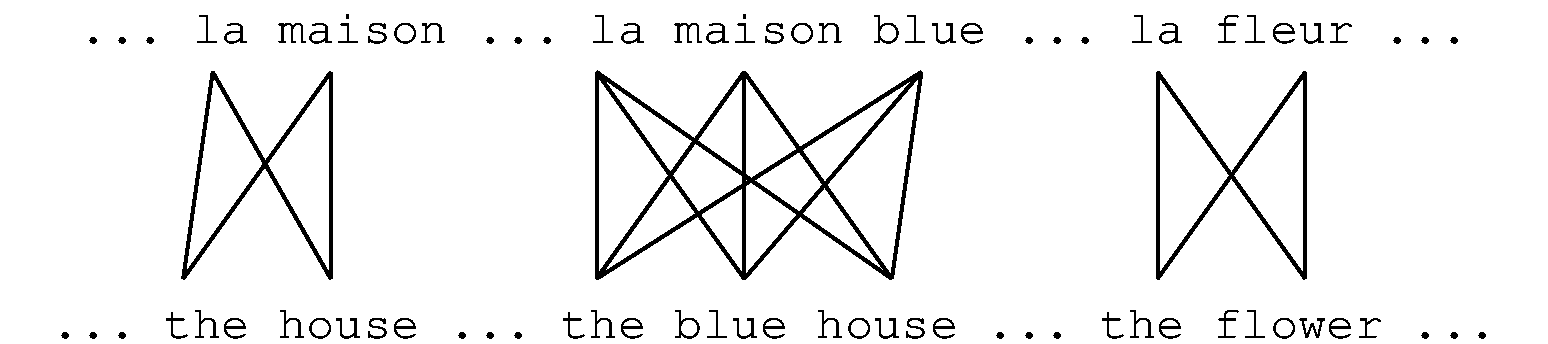
\includegraphics[scale=0.9]{em1.pdf}
\end{center}
\begin{itemize}
\item Initial step: all alignments equally likely
\item Model learns that, e.g., \example{la} is often aligned with \example{the}
\end{itemize}


%%%%%%%%%%%%%%%%%%%%%%%%%%%%%%%%%%%%%%%%%%%%%%%%%%%%%%%%%%%%%%%%%%%%%%%%%%%%

\slide{EM Algorithm}
\vspace{10mm}
\begin{center}

\includegraphics[scale=0.9]{em2.pdf}
\end{center}
\begin{itemize}
\item After one iteration
\item Alignments, e.g., between \example{la} and \example{the} are more likely
\end{itemize}


%%%%%%%%%%%%%%%%%%%%%%%%%%%%%%%%%%%%%%%%%%%%%%%%%%%%%%%%%%%%%%%%%%%%%%%%%%%%

\slide{EM Algorithm}
\vspace{10mm}
\begin{center}
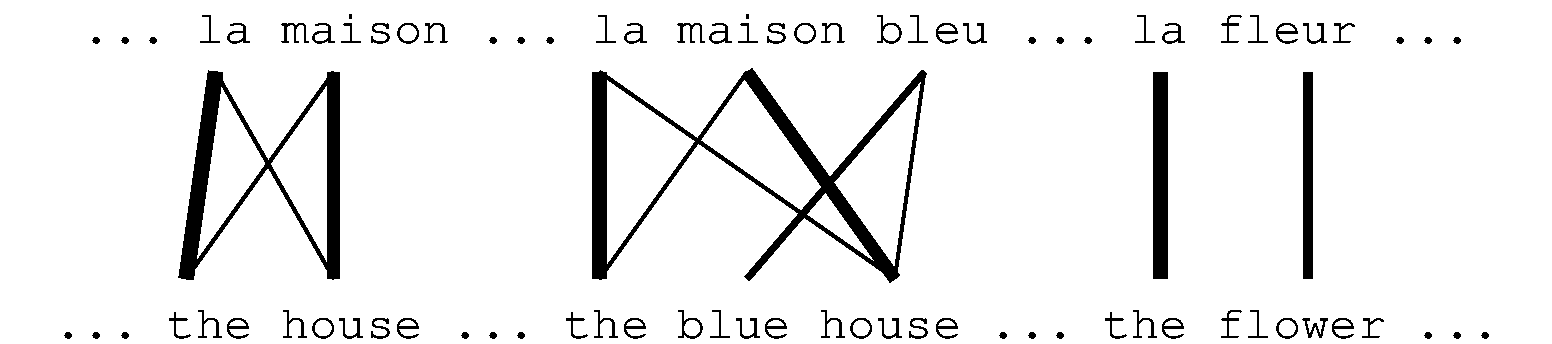
\includegraphics[scale=0.9]{em3.pdf}
\end{center}
\begin{itemize}
\item After another iteration
\item It becomes apparent that alignments, e.g., between \example{fleur}
  and \example{flower} are more likely (pigeon hole principle)
\end{itemize}


%%%%%%%%%%%%%%%%%%%%%%%%%%%%%%%%%%%%%%%%%%%%%%%%%%%%%%%%%%%%%%%%%%%%%%%%%%%%

\slide{EM Algorithm}
\vspace{10mm}
\begin{center}
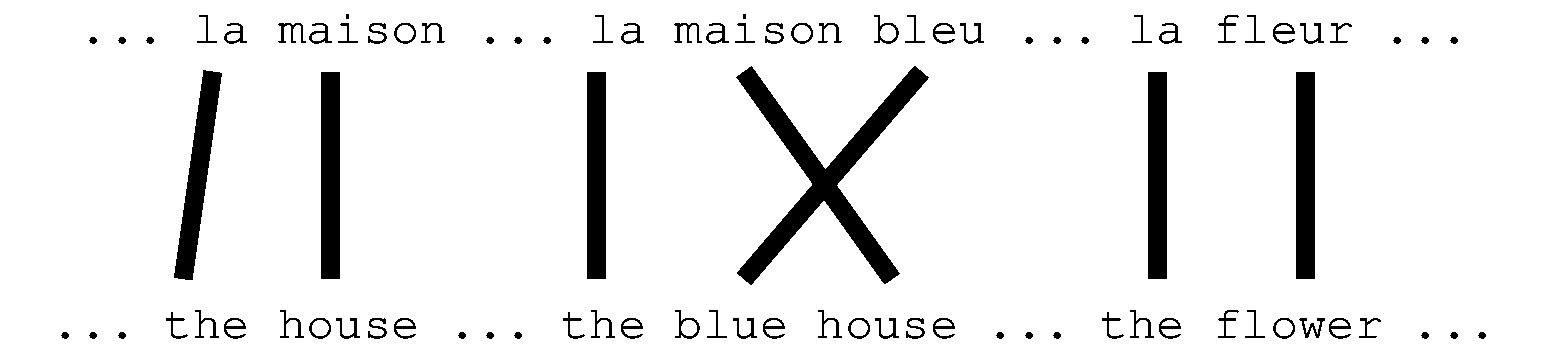
\includegraphics[scale=0.9]{em4.pdf}
\end{center}
\begin{itemize}
\item Convergence
\item Inherent hidden structure revealed by EM
\end{itemize}


%%%%%%%%%%%%%%%%%%%%%%%%%%%%%%%%%%%%%%%%%%%%%%%%%%%%%%%%%%%%%%%%%%%%%%%%%%%%

\slide{EM Algorithm}
\vspace{5mm}
\begin{center}
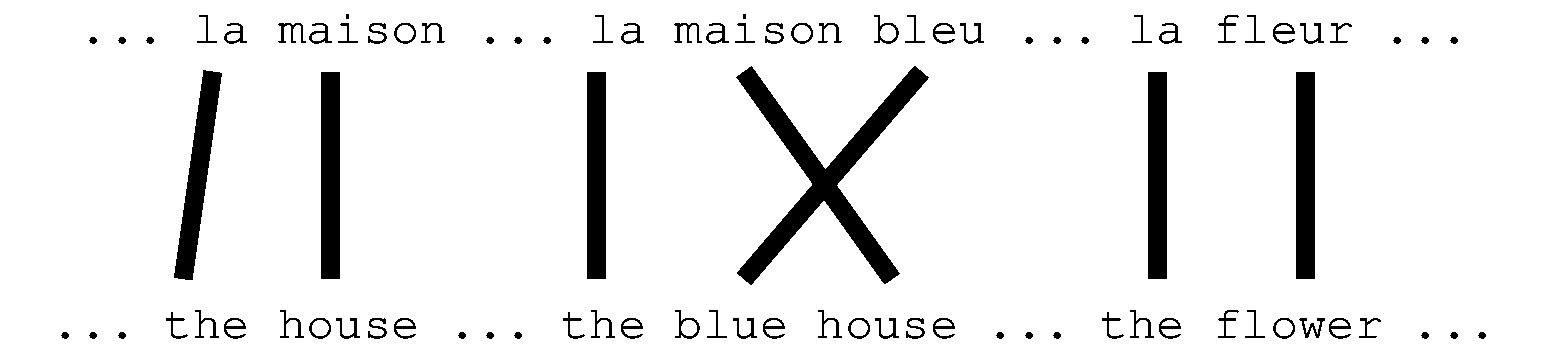
\includegraphics[scale=0.9]{em4.pdf}
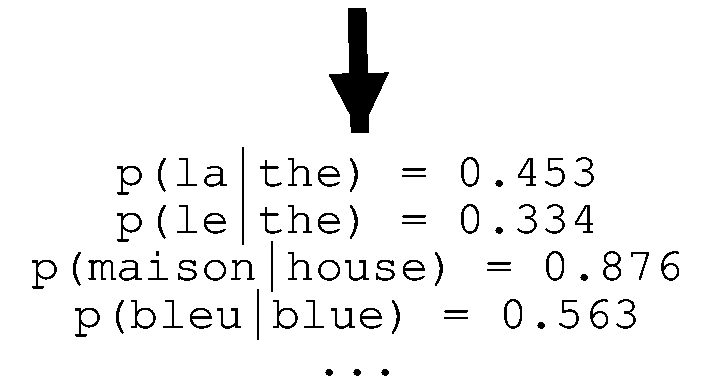
\includegraphics[scale=0.9]{em-result.pdf}
\end{center}
\begin{itemize}
\item Parameter estimation from the aligned corpus
\end{itemize}


%%%%%%%%%%%%%%%%%%%%%%%%%%%%%%%%%%%%%%%%%%%%%%%%%%%%%%%%%%%%%%%%%%%%%%%%%%%%

\slide{IBM Model 1 and EM}
\vspace{5mm}
\begin{itemize}
\item EM Algorithm consists of two steps
\item Expectation-Step: Apply model to the data
\begin{itemize}
\item parts of the model are hidden (here: alignments)
\item using the model, assign probabilities to possible values
\end{itemize}
\item Maximization-Step: Estimate model from data
\begin{itemize}
\item take assign values as fact
\item collect counts (weighted by probabilities)
\item estimate model from counts
\end{itemize}
\item Iterate these steps until convergence
\end{itemize}


%%%%%%%%%%%%%%%%%%%%%%%%%%%%%%%%%%%%%%%%%%%%%%%%%%%%%%%%%%%%%%%%%%%%%%%%%%%%

\slide{IBM Model 1 and EM}
\vspace{30mm}
\begin{itemize}
\item We need to be able to compute:\vspace{10mm}
\begin{itemize}
\item Expectation-Step: probability of alignments\vspace{10mm}
\item Maximization-Step: count collection
\end{itemize}
\end{itemize}


%%%%%%%%%%%%%%%%%%%%%%%%%%%%%%%%%%%%%%%%%%%%%%%%%%%%%%%%%%%%%%%%%%%%%%%%%%%%

\slide{IBM Model 1 and EM}
\vspace{10mm}
\begin{itemize}
\item {\bf Probabilities} \hspace{2cm}
\maths{\begin{tabular}{cc}
$p(\text{\example{the}}|\text{\example{la}}) = 0.7$ &
$p(\text{\example{house}}|\text{\example{la}}) = 0.05$ \\
$p(\text{\example{the}}|\text{\example{maison}}) = 0.1$ &
$p(\text{\example{house}}|\text{\example{maison}}) = 0.8$
\end{tabular}}
\item {\bf Alignments}\\
\begin{tabular}{cccc}
\example{\begin{bipartite}{2cm}{15mm}{15mm}{3mm}{3mm}
\leftnode{la} \leftnode{maison} 
\rightnode{the} \rightnode{house}
\match{la}{the}
\match{maison}{house}
\end{bipartite}}
&
\example{\begin{bipartite}{2cm}{15mm}{15mm}{3mm}{3mm}
\leftnode{la} \leftnode{maison} 
\rightnode{the} \rightnode{house}
\match{la}{the}
\match{la}{house}
\end{bipartite}}
&
\example{\begin{bipartite}{2cm}{15mm}{15mm}{3mm}{3mm}
\leftnode{la} \leftnode{maison} 
\rightnode{the} \rightnode{house}
\match{maison}{the}
\match{maison}{house}
\end{bipartite}}
&
\example{\begin{bipartite}{2cm}{15mm}{15mm}{3mm}{3mm}
\leftnode{la} \leftnode{maison} 
\rightnode{the} \rightnode{house}
\match{la}{house}
\match{maison}{the}
\end{bipartite}} \\ 
& & & \\
\maths{$p({\bf e},a|{\bf f}) = 0.56$} &
\maths{$p({\bf e},a|{\bf f}) = 0.035$} &
\maths{$p({\bf e},a|{\bf f}) = 0.08$} &
\maths{$p({\bf e},a|{\bf f}) = 0.005$} \\
& & & \\
\maths{$p(a|{\bf e},{\bf f}) = 0.824$} & 
\maths{$p(a|{\bf e},{\bf f}) = 0.052$} & 
\maths{$p(a|{\bf e},{\bf f}) = 0.118$} & 
\maths{$p(a|{\bf e},{\bf f}) = 0.007$}
\end{tabular}
\item {\bf Counts} 
\maths{\begin{tabular}{cc}
$c(\text{\example{the}}|\text{\example{la}}) = 0.824+0.052$ &
$c(\text{\example{house}}|\text{\example{la}}) = 0.052+0.007$ \\
$c(\text{\example{the}}|\text{\example{maison}}) = 0.118+0.007$ &
$c(\text{\example{house}}|\text{\example{maison}}) = 0.824+0.118$
\end{tabular}}
\end{itemize}


%%%%%%%%%%%%%%%%%%%%%%%%%%%%%%%%%%%%%%%%%%%%%%%%%%%%%%%%%%%%%%%%%%%%%%%%%%%%

\slide{IBM Model 1 and EM: Expectation Step}
\vspace{20mm}
\begin{itemize}
\item We need to compute \maths{$p(a|\mbox{\bf e},\mbox{\bf f})$}
\item Applying the chain rule:
\end{itemize}
\maths{\begin{equation*}
p(a|\mbox{\bf e},\mbox{\bf f}) =
\frac{p(\mbox{\bf e},a|\mbox{\bf f})}
{p(\mbox{\bf e}|\mbox{\bf f})}
\label{eqn:wb:p_a}
\end{equation*}}
\begin{itemize}
\item We already have the formula for \maths{$p(\mbox{\bf e},\mbox{\bf a}|\mbox{\bf f})$} (definition of Model 1)
\end{itemize}


%%%%%%%%%%%%%%%%%%%%%%%%%%%%%%%%%%%%%%%%%%%%%%%%%%%%%%%%%%%%%%%%%%%%%%%%%%%%

\slide{IBM Model 1 and EM: Expectation Step}
\vspace{10mm}
\begin{itemize}
\item We need to compute \maths{$p(\mbox{\bf e}|\mbox{\bf f})$}
\end{itemize}
\maths{\begin{equation*}
\begin{split}
p({\bf e}|{\bf f}) &= \sum_a p({\bf e},a|{\bf f}) \\
&= \sum_{a(1)=0}^{l_f} ... \sum_{a(l_e)=0}^{l_f} p({\bf e},a|{\bf f})\\
&= \sum_{a(1)=0}^{l_f} ... \sum_{a(l_e)=0}^{l_f} 
\frac{\epsilon}{(l_f+1)^{l_e}} \prod_{j=1}^{l_e} t(e_j|f_{a(j)}) \\
\end{split}
\end{equation*}}


%%%%%%%%%%%%%%%%%%%%%%%%%%%%%%%%%%%%%%%%%%%%%%%%%%%%%%%%%%%%%%%%%%%%%%%%%%%%

\slide{IBM Model 1 and EM: Expectation Step}
\vspace{5mm}
\maths{\begin{equation*}
\begin{split}
p({\bf e}|{\bf f})
&= \sum_{a(1)=0}^{l_f} ... \sum_{a(l_e)=0}^{l_f} 
\frac{\epsilon}{(l_f+1)^{l_e}} \prod_{j=1}^{l_e} t(e_j|f_{a(j)}) \\
&= \frac{\epsilon}{{(l_f+1)}^{l_e}}  \sum_{a(1)=0}^{l_f} ... \sum_{a(l_e)=0}^{l_f}
\prod_{j=1}^{l_e} t(e_j|f_{a(j)}) \\
&= \frac{\epsilon}{{(l_f+1)}^{l_e}} \prod_{j=1}^{l_e} \sum_{i=0}^{l_f} t(e_j|f_i)
\end{split}
\end{equation*}}
\begin{itemize}
\item Note the trick in the last line 
\begin{itemize} 
\item removes the need for an exponential number of products 
\item[$\rightarrow$] this makes IBM Model 1 estimation tractable
\end{itemize}
\end{itemize}


%%%%%%%%%%%%%%%%%%%%%%%%%%%%%%%%%%%%%%%%%%%%%%%%%%%%%%%%%%%%%%%%%%%%%%%%%%%%

\slide{The Trick}
\begin{center}
(case \maths{$l_e=l_f=2$}) 
\end{center}
\maths{\begin{equation*}
\begin{split}
\sum_{a(1)=0}^2 \sum_{a(2)=0}^2 =
& \; \frac{\epsilon}{3^2} \prod_{j=1}^2 t(e_j|f_{a(j)}) =\\
= & \; t(e_1|f_0)\;t(e_2|f_0)
+ t(e_1|f_0)\;t(e_2|f_1)
+ t(e_1|f_0)\;t(e_2|f_2) +\\
& + t(e_1|f_1)\;t(e_2|f_0)
+ t(e_1|f_1)\;t(e_2|f_1)
+ t(e_1|f_1)\;t(e_2|f_2) +\\
& + t(e_1|f_2)\;t(e_2|f_0)
+ t(e_1|f_2)\;t(e_2|f_1)
+ t(e_1|f_2)\;t(e_2|f_2) = \\
= & \; t(e_1|f_0) \left( t(e_2|f_0) + t(e_2|f_1) + t(e_2|f_2) \right) +\\
& + t(e_1|f_1) \left( t(e_2|f_1) + t(e_2|f_1) + t(e_2|f_2) \right) +\\
& + t(e_1|f_2) \left( t(e_2|f_2) + t(e_2|f_1) + t(e_2|f_2) \right) =\\
= & \; \left( t(e_1|f_0) + t(e_1|f_1) + t(e_1|f_2) \right)
\left( t(e_2|f_2) + t(e_2|f_1) + t(e_2|f_2) \right)
\end{split}
\end{equation*}}



%%%%%%%%%%%%%%%%%%%%%%%%%%%%%%%%%%%%%%%%%%%%%%%%%%%%%%%%%%%%%%%%%%%%%%%%%%%%

\slide{IBM Model 1 and EM: Expectation Step}
\vspace{10mm}\begin{itemize}
\item Combine what we have:
\end{itemize}
\vspace{5mm}
\maths{\begin{equation*}
\begin{split}
p(\mbox{\bf a}|\mbox{\bf e},\mbox{\bf f}) &=
p(\mbox{\bf e},\mbox{\bf a}|\mbox{\bf f}) /
p(\mbox{\bf e}|\mbox{\bf f}) \\[3mm]
&= \frac{\frac{\epsilon}{(l_f+1)^{l_e}} \prod_{j=1}^{l_e}
  t(e_j|f_{a(j)})}{\frac{\epsilon}{(l_f+1)^{l_e}} \prod_{j=1}^{l_e} \sum_{i=0}^{l_f} t(e_j|f_i)} \\
&= \prod_{j=1}^{l_e} \frac{t(e_j|f_{a(j)})}{\sum_{i=0}^{l_f} t(e_j|f_i)}
\end{split}
\end{equation*}}


%%%%%%%%%%%%%%%%%%%%%%%%%%%%%%%%%%%%%%%%%%%%%%%%%%%%%%%%%%%%%%%%%%%%%%%%%%%%

\slide{IBM Model 1 and EM: Maximization Step}
\begin{itemize}
\item Now we have to collect counts
\item Evidence from a sentence pair \maths{{\bf e,f}} that word \maths{$e$} is a
  translation of word \maths{$f$}:
\end{itemize}
\maths{\begin{equation*}
c(e|f;{\bf e},{\bf f}) = \sum_{a} 
p(a|{\bf e},{\bf f}) 
\sum_{j=1}^{l_e} \delta(e,e_j) \delta(f,f_{a(j)})
\end{equation*}}
\begin{itemize}
\item With the same simplication as before:
\end{itemize}
\maths{\begin{equation*}
c(e|f;{\bf e},{\bf f}) = \frac{t(e|f)}{\sum_{i=0}^{l_f} t(e|f_i)}
\sum_{j=1}^{l_e} \delta(e,e_j) \sum_{i=0}^{l_f} \delta(f,f_i)
\end{equation*}}


%%%%%%%%%%%%%%%%%%%%%%%%%%%%%%%%%%%%%%%%%%%%%%%%%%%%%%%%%%%%%%%%%%%%%%%%%%%%

\slide{IBM Model 1 and EM: Maximization Step}
\vspace{30mm}
\begin{center}
After collecting these counts over a corpus, we can estimate the model:
\end{center}
\vspace{10mm}
\maths{\begin{equation*}
t(e|f;\mbox{\bf e},\mbox{\bf f}) = 
\frac{\sum_{(\mbox{\bf e},\mbox{\bf f})} c(e|f;\mbox{\bf e},\mbox{\bf f}))}
{\sum_e \sum_{(\mbox{\bf e},\mbox{\bf f})} c(e|f;\mbox{\bf e},\mbox{\bf f}))}
\end{equation*}}


%%%%%%%%%%%%%%%%%%%%%%%%%%%%%%%%%%%%%%%%%%%%%%%%%%%%%%%%%%%%%%%%%%%%%%%%%%%%

\slide{IBM Model 1 and EM: Pseudocode}
\begin{center} \vspace{-1mm}
\begin{multicols}{2}
\begin{algorithmic}[1]
\REQUIRE set of sentence pairs $(\text{\bf e},\text{\bf f})$
\ENSURE translation prob. $t(e|f)$
\STATE initialize $t(e|f)$ uniformly
\WHILE{not converged}
  \STATE \COMMENT{initialize}
  \STATE count($e|f$) = 0 {\bf for all} $e,f$
  \STATE total($f$) = 0 {\bf for all} $f$
  \FORALL{sentence pairs ({\bf e},{\bf f})}
    \STATE \COMMENT{compute normalization}
    \FORALL{words $e$ in {\bf e}}
      \STATE s-total($e$) = 0
      \FORALL{words $f$ in {\bf f}}
        \STATE s-total($e$) += $t(e|f)$
      \ENDFOR
    \ENDFOR
    \STATE \COMMENT{collect counts}
    \FORALL{words $e$ in {\bf e}}
      \FORALL{words $f$ in {\bf f}}
        \STATE count($e|f$) += $\frac{t(e|f)}{\text{s-total}(e)}$
        \STATE total($f$)   += $\frac{t(e|f)}{\text{s-total}(e)}$
      \ENDFOR
    \ENDFOR
  \ENDFOR
  \STATE \COMMENT{estimate probabilities}
  \FORALL{foreign words $f$}
    \FORALL{English words $e$}
      \STATE $t(e|f)$ = $\frac{\text{count}(e|f)}{\text{total}(f)}$
    \ENDFOR
  \ENDFOR
\ENDWHILE
\end{algorithmic}
\end{multicols}
\end{center}


%%%%%%%%%%%%%%%%%%%%%%%%%%%%%%%%%%%%%%%%%%%%%%%%%%%%%%%%%%%%%%%%%%%%%%%%%%%%

\slide{Convergence}
\begin{center}\vspace{-3mm}
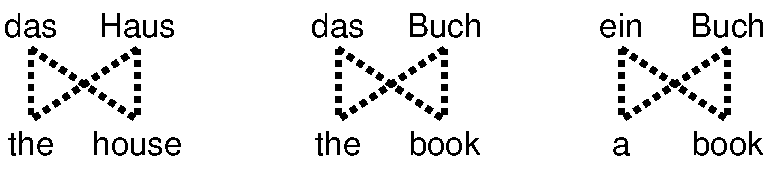
\includegraphics[scale=1.2]{em-model1-corpus.pdf}
\begin{tabular}{|c|c||c|c|c|c|c|c|} \hline
$e$ & $f$ & initial & 1st it. & 2nd it. & 3rd it. & ... & final \\ \hline \hline
\example{the} & \example{das} & 0.25 & 0.5 & 0.6364 & 0.7479 & ... & 1 \\ \hline
\example{book} & \example{das} & 0.25 & 0.25 & 0.1818 & 0.1208 & ... & 0 \\ \hline
\example{house} & \example{das} & 0.25 & 0.25 & 0.1818 & 0.1313 & ... &0 \\ \hline
\example{the} & \example{buch} & 0.25 & 0.25 & 0.1818 & 0.1208 & ... & 0 \\ \hline
\example{book} & \example{buch} & 0.25 & 0.5 & 0.6364 & 0.7479 & ... & 1 \\ \hline 
\example{a} & \example{buch} & 0.25 & 0.25 & 0.1818 & 0.1313 & ... & 0 \\ \hline
\example{book} & \example{ein} & 0.25 & 0.5 & 0.4286 & 0.3466 & ...&  0 \\ \hline
\example{a} & \example{ein} & 0.25 & 0.5 &  0.5714 & 0.6534 & ...& 1 \\ \hline
\example{the} & \example{haus} & 0.25 & 0.5 &  0.4286 & 0.3466 & ...&  0 \\ \hline
\example{house} & \example{haus} & 0.25 & 0.5 &  0.5714 & 0.6534 & ...& 1 \\ \hline
\end{tabular}
\end{center}



%%%%%%%%%%%%%%%%%%%%%%%%%%%%%%%%%%%%%%%%%%%%%%%%%%%%%%%%%%%%%%%%%%%%%%%%%%%%

\slide{Perplexity}
\begin{itemize} 
\item How well does the model fit the data?
\item Perplexity: derived from probability of the training data according to the model
\maths{\begin{equation*}
\log_2 PP = -\sum_s \log_2 p({\bf e}_s |{\bf f}_s )
\end{equation*}}\vspace{-10mm}
\item Example (\maths{$\epsilon$=1})\\[10mm]
\begin{tabular}{|c|l|l|l|l|l|l|} \hline
& initial & 1st it. & 2nd it. & 3rd it. & ... & final \\ \hline
\maths{$p(\text{\example{the haus}}|\text{\example{das haus}})$} & 0.0625 & 0.1875 & 0.1905 & 0.1913 &...& 0.1875\\ \hline
\maths{$p(\text{\example{the book}}|\text{\example{das buch}})$} & 0.0625 & 0.1406 & 0.1790 & 0.2075 &...& 0.25  \\ \hline
\maths{$p(\text{\example{a book}}|\text{\example{ein buch}})$}   & 0.0625 & 0.1875 & 0.1907 & 0.1913 &...& 0.1875\\ \hline
perplexity & 4095 & 202.3 & 153.6 & 131.6 & ... & 113.8 \\ \hline
\end{tabular}
\end{itemize}

%%%%%%%%%%%%%%%%%%%%%%%%%%%%%%%%%%%%%%%%%%%%%%%%%%%%%%%%%%%%%%%%%%%%%%%%%%%%

\slide{Ensuring Fluent Output}
\begin{itemize}
\item Our translation model cannot decide between \example{small} and \example{little}
\item Sometime one is preferred over the other:
\begin{itemize}
\item \example{small step}: 2,070,000 occurrences in the Google index 
\item \example{little step}: 257,000 occurrences in the Google index 
\end{itemize}
\item Language model
\begin{itemize}
\item estimate how likely a string is English
\item based on n-gram statistics
\end{itemize}
\maths{\begin{equation*}
\begin{split}
p({\bf e}) &= p(e_1,e_2,...,e_n) \\
 &= p(e_1) p(e_2|e_1) ... p(e_n|e_1,e_2,...,e_{n-1}) \\
 &\simeq p(e_1) p(e_2|e_1) ... p(e_n|e_{n-2},e_{n-1})
\end{split}
\end{equation*}}
\end{itemize}

%%%%%%%%%%%%%%%%%%%%%%%%%%%%%%%%%%%%%%%%%%%%%%%%%%%%%%%%%%%%%%%%%%%%%%%%%%%%

\slide{Noisy Channel Model}
\begin{itemize}\vspace{20mm}
\item We would like to integrate a language model
\item Bayes rule
\maths{\begin{equation*}
\begin{split}
\mbox{argmax}_{\bf e} \; p({\bf e}|{\bf f}) &= \mbox{argmax}_{\bf e} \frac{p({\bf f}|{\bf e}) \; p({\bf e})}{p({\bf f})} \\
&= \mbox{argmax}_{\bf e} \; p({\bf f}|{\bf e}) \; p({\bf e})
\end{split}
\end{equation*}}
\end{itemize}

%%%%%%%%%%%%%%%%%%%%%%%%%%%%%%%%%%%%%%%%%%%%%%%%%%%%%%%%%%%%%%%%%%%%%%%%%%%%

\slide{Noisy Channel Model}
\vspace{10mm}
\begin{center}
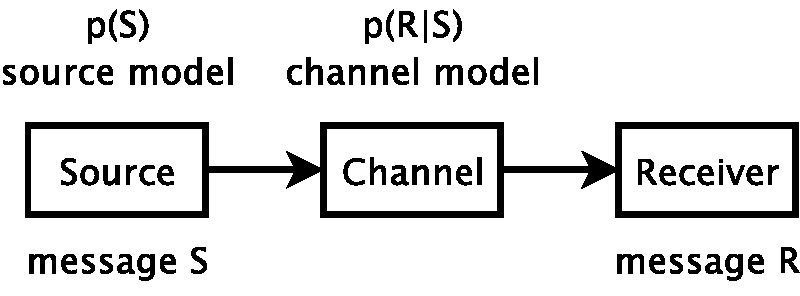
\includegraphics[scale=1.1]{noisy-channel.pdf}
\end{center}
\vspace{5mm}
\begin{itemize}
\item Applying Bayes rule also called noisy channel model
\begin{itemize}
\item we observe a distorted message R (here: a foreign string \maths{\bf f})
\item we have a model on how the message is distorted (here: translation model)
\item we have a model on what messages are probably (here: language model)
\item we want to recover the original message S (here: an English string \maths{\bf e})
\end{itemize}
\end{itemize}

%%%%%%%%%%%%%%%%%%%%%%%%%%%%%%%%%%%%%%%%%%%%%%%%%%%%%%%%%%%%%%%%%%%%%%%%%%%%

\slide{Higher IBM Models}
\vspace{10mm}
\begin{center}
\begin{tabular}{|l|l|} \hline
IBM Model 1 & lexical translation \\ \hline
IBM Model 2 & adds absolute reordering model \\ \hline
IBM Model 3 & adds fertility model \\ \hline
IBM Model 4 & relative reordering model \\ \hline
IBM Model 5 & fixes deficiency \\ \hline
\end{tabular}
\end{center}
\begin{itemize}
\item Only IBM Model 1 has global maximum \vspace{-3mm}
\begin{itemize}
\item training of a higher IBM model builds on previous model
\end{itemize}
\item Compuationally biggest change in Model 3 \vspace{-3mm}
\begin{itemize} 
\item trick to simplify estimation does not work anymore
\item[$\rightarrow$] exhaustive count collection becomes computationally too expensive
\item sampling over high probability alignments is used instead
\end{itemize}
\end{itemize}


%%%%%%%%%%%%%%%%%%%%%%%%%%%%%%%%%%%%%%%%%%%%%%%%%%%%%%%%%%%%%%%%%%%%%%%%%%%%

\slide{Reminder: IBM Model 1}
\begin{itemize}
\item Generative model: break up translation process into smaller steps
\begin{itemize} \vspace{-3mm}
\item IBM Model 1 only uses lexical translation
\end{itemize} 
\item Translation probability 
\begin{itemize} \vspace{-3mm}
\item for a foreign sentence \maths{{\bf f} $= (f_1, ..., f_{l_f})$} of length  \maths{$l_f$}
\item to an English sentence  \maths{{\bf e} $= (e_1, ..., e_{l_e})$} of length  \maths{$l_e$} 
\item with an alignment of each English word  \maths{$e_j$} to a foreign word  \maths{$f_i$} according to the alignment function  \maths{$a: j \rightarrow i$}
 \maths{\begin{equation*}
p({\bf e},a|{\bf f}) = 
\frac{\epsilon}{(l_f+1)^{l_e}} \prod_{j=1}^{l_e} t(e_j|f_{a(j)})
\end{equation*}}
\item parameter  \maths{$\epsilon$} is a normalization constant
\end{itemize}
\end{itemize}

%%%%%%%%%%%%%%%%%%%%%%%%%%%%%%%%%%%%%%%%%%%%%%%%%%%%%%%%%%%%%%%%%%%%%%%%%%%%

\slide{IBM Model 2}
\vspace{20mm}
\begin{center} 
Adding a model of alignment\\[10mm]
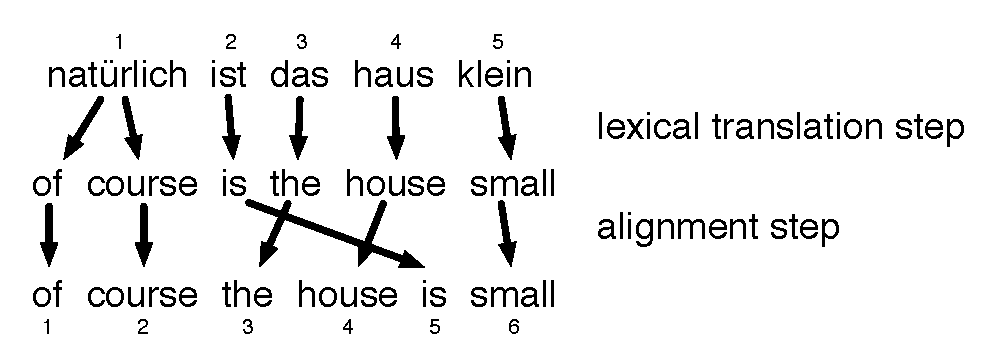
\includegraphics[scale=1.3]{natuerlich-haus-klein-model2.pdf}
\end{center}

\slide{IBM Model 2}
\begin{itemize}
\item Modeling alignment with an alignment probability distribution
\item Translating foreign word at position \maths{$i$} to English word at position \maths{$j$}:
\maths{\begin{equation*}\vspace{-5mm}
a(i|j,l_e,l_f)
\end{equation*}}\vspace{-5mm}
\item Putting everything together
\maths{\begin{equation*}\vspace{-10mm}
p({\bf e},a|{\bf f}) = 
\epsilon \prod_{j=1}^{l_e} t(e_j|f_{a(j)}) \; a(a(j)|j,l_e,l_f)
\end{equation*}}\vspace{-5mm}
\item EM training of this model works the same way as IBM Model 1
\end{itemize}

%%%%%%%%%%%%%%%%%%%%%%%%%%%%%%%%%%%%%%%%%%%%%%%%%%%%%%%%%%%%%%%%%%%%%%%%%%%%

\slide{Interlude: HMM Model}
\vspace{10mm}
\begin{itemize}
\item Words do not move independently of each other
\begin{itemize}
\item they often move in groups
\item[$\rightarrow$] condition word movements on previous word
\end{itemize} 
\item HMM alignment model:\\
\maths{\begin{equation*}
p(a(j)|a(j-1),l_e)
\end{equation*}}
\item EM algorithm application harder, requires dynamic programming
\item IBM Model 4 is similar, also conditions on word classes
\end{itemize}


%%%%%%%%%%%%%%%%%%%%%%%%%%%%%%%%%%%%%%%%%%%%%%%%%%%%%%%%%%%%%%%%%%%%%%%%%%%%

\slide{IBM Model 3}
\begin{center} 
Adding a model of fertilty\\[10mm]
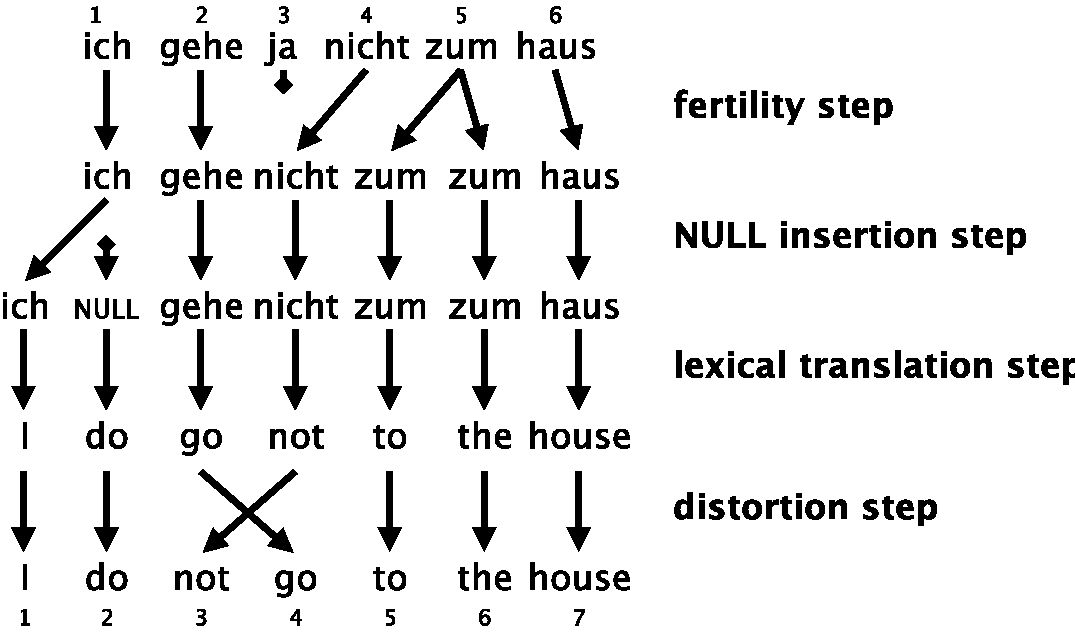
\includegraphics[scale=1.0]{ich-gehe-ja-nicht-model3.pdf}
\end{center}

%%%%%%%%%%%%%%%%%%%%%%%%%%%%%%%%%%%%%%%%%%%%%%%%%%%%%%%%%%%%%%%%%%%%%%%%%%%%

\slide{IBM Model 3: Fertility}
\vspace{10mm}
\begin{itemize}
\item Fertility: number of English words generated by a foreign word
\item Modelled by distribution \maths{$n(\phi|f)$}
\item Example:
\maths{\begin{equation*}
\begin{split}
n(1|\text{\example{haus}}) \simeq 1\\
n(2|\text{\example{zum}}) \simeq 1\\
n(0|\text{\example{ja}}) \simeq 1
\end{split}
\end{equation*}}
\end{itemize}

%%%%%%%%%%%%%%%%%%%%%%%%%%%%%%%%%%%%%%%%%%%%%%%%%%%%%%%%%%%%%%%%%%%%%%%%%%%%

\slide{Sampling the Alignment Space}
\begin{itemize}
\item Training IBM Model 3 with the EM algorithm
\begin{itemize}
\item The trick that reduces exponential complexity does not work anymore
\item[$\rightarrow$] Not possible to exhaustively consider all alignments
\end{itemize}
\item Finding the most probable alignment by hillclimbing
\begin{itemize}
\item start with initial alignment
\item change alignments for individual words
\item keep change if it has higher probability
\item continue until convergence
\end{itemize}
\item Sampling: collecting variations to collect statistics
\begin{itemize}
\item all alignments found during hillclimbing
\item neighboring alignments that differ by a move or a swap
\end{itemize}
\end{itemize}
 
%%%%%%%%%%%%%%%%%%%%%%%%%%%%%%%%%%%%%%%%%%%%%%%%%%%%%%%%%%%%%%%%%%%%%%%%%%%%

\slide{IBM Model 4}
\vspace{20mm}
\begin{itemize}
\item Better reordering model
\item Reordering in IBM Model 2 and 3 
\begin{itemize}
\item recall: \maths{$d(j | |_i, l_e , lf )$}
\item for large sentences (large \maths{$l_f$} and  \maths{$l_e$}), sparse and unreliable statistics
\item phrases tend to move together
\end{itemize}
\item Relative reordering model: relative to previously translated words (cepts)
\end{itemize}

%%%%%%%%%%%%%%%%%%%%%%%%%%%%%%%%%%%%%%%%%%%%%%%%%%%%%%%%%%%%%%%%%%%%%%%%%%%%

\slide{IBM Model 4: Cepts}
\begin{center}
Foreign words with non-zero fertility forms cepts\\
(here 5 cepts)\\[10mm]
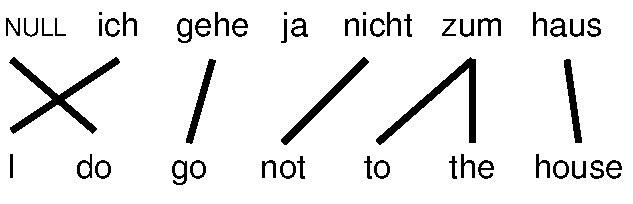
\includegraphics[scale=1.2]{ich-gehe-ja-nicht-alignment.pdf}\\[10mm]
\begin{tabular}{|c||c|c|c|c|c|} \hline
cept \maths{$\pi_i$} & \maths{$\pi_1$} & \maths{$\pi_2$} & \maths{$\pi_3$} & \maths{$\pi_4$} & \maths{$\pi_5$} \\ \hline
foreign position \maths{$[i]$} & 1 & 2 & 4 & 5 & 6 \\ \hline
foreign word \maths{$f_{[i]}$} & \example{ich} & \example{gehe} & \example{nicht} & \example{zum} & \example{haus} \\ \hline
English words \maths{$\{e_j\}$} & \example{I} & \example{go} & \example{not} & \example{to},\example{the} & \example{house} \\ \hline
English positions \maths{$\{j\}$} & 1 & 4 & 3 & 5,6 & 7 \\ \hline
center of cept \maths{$\odot_i$} & 1 & 4 & 3 & 6 & 7 \\ \hline
\end{tabular}
\end{center}

%%%%%%%%%%%%%%%%%%%%%%%%%%%%%%%%%%%%%%%%%%%%%%%%%%%%%%%%%%%%%%%%%%%%%%%%%%%%

\slide{IBM Model 4: Relative Distortion}
\vspace{10mm}
\begin{tabular}{|c||c|c|c|c|c|c|c|c|} \hline
\maths{$j$} & 1 & 2 & 3 & 4 & 5 & 6 & 7 \\ \hline
\maths{$e_j$} & \example{I} & \example{do} & \example{not} & \example{go} & \example{to} & \example{the} & \example{house} \\\hline
in cept \maths{$\pi_{i,k}$} & \maths{$\pi_{1,0}$} & \maths{$\pi_{0,0}$} & \maths{$\pi_{3,0}$} & \maths{$\pi_{2,0}$} & \maths{$\pi_{4,0}$} & \maths{$\pi_{4,1}$} & \maths{$\pi_{5,0}$} \\ \hline
\maths{$\odot_{i-1}$}   & 0 & - & 4 & 1 & 3 & - & 6 \\ \hline
\maths{$j-\odot_{i-1}$} & $+1$ & - & $-1$ & $+3$ & $+2$ & - & $+1$ \\ \hline
distortion & \maths{$d_1(+1)$} & 1 & \maths{$d_1(-1)$} & \maths{$d_1(+3)$} & \maths{$d_1(+2)$} & \maths{$d_{>1}(+1)$} & \maths{$d_1(+1)$} \\ \hline 
\end{tabular}
\vspace{5mm}
\begin{itemize}
\item Center \maths{$\odot_i$} of a cept \maths{$\pi_i$} is \maths{$\text{ceiling}(\text{avg}(j))$}
\item Three cases:
\begin{itemize}
\item uniform for {\sc null} generated words
\item first word of a cept: \maths{$d_1$}
\item next words of a cept: \maths{$d_{>1}$}
\end{itemize}
\end{itemize}


%%%%%%%%%%%%%%%%%%%%%%%%%%%%%%%%%%%%%%%%%%%%%%%%%%%%%%%%%%%%%%%%%%%%%%%%%%%%

\slide{Word Classes}
\vspace{10mm}
\begin{itemize}
\item Some words may trigger reordering
$\rightarrow$ condition reordering on words
\maths{\begin{equation*}
\begin{split}
\mbox{\textcolor{black}{for initial word in cept:}}
& \; \; \; d_1(j-\odot_{[i-1]}|f_{[i-1]},e_j) \\
\mbox{\textcolor{black}{for additional words:}}
& \; \; \; d_{>1}(j-\Pi_{i,k-1}|e_j) 
\end{split}
\label{eqn:eb:model4-distortion-lex}
\end{equation*}}
\item Sparse data concerns $\rightarrow$ cluster words into classes
\maths{\begin{equation*}
\begin{split}
\mbox{\textcolor{black}{for initial word in cept:}}
& \; \; \; d_1(j-\odot_{[i-1]}|\mathcal{A}(f_{[i-1]}),\mathcal{B}(e_j)) \\
\mbox{\textcolor{black}{for additional words:}}
& \; \; \; d_{>1}(j-\Pi_{i,k-1}|\mathcal{B}(e_j)) 
\end{split}
\end{equation*}}
\end{itemize}

%%%%%%%%%%%%%%%%%%%%%%%%%%%%%%%%%%%%%%%%%%%%%%%%%%%%%%%%%%%%%%%%%%%%%%%%%%%%

\slide{IBM Model 5}
\vspace{20mm}
\begin{itemize}
\item IBM Models 1--4 are {\em deficient}
\begin{itemize} \itemsep 2mm
\item some impossible translations have positive probability
\item multiple output words may be placed in the same position
\item[$\rightarrow$] probability mass is wasted
\end{itemize}
\vspace{10mm}
\item IBM Model 5 fixes deficiency by keeping track of vacancies (available positions)
\end{itemize}

%%%%%%%%%%%%%%%%%%%%%%%%%%%%%%%%%%%%%%%%%%%%%%%%%%%%%%%%%%%%%%%%%%%%%%%%%%%%

\slide{Conclusion}
\vspace{10mm}
\begin{itemize}
\item IBM Models were the pioneering models in statistical machine translation
\item Introduced important concepts
\begin{itemize}
\item generative model
\item EM training
\item reordering models
\end{itemize}
\vspace{5mm}
\item Only used for niche applications as translation model
\item ... but still in common use for word alignment (e.g., GIZA++ toolkit)
\end{itemize}

%%%%%%%%%%%%%%%%%%%%%%%%%%%%%%%%%%%%%%%%%%%%%%%%%%%%%%%%%%%%%%%%%%%%%%%%%%%%

\slide{Word Alignment}
\vspace{5mm}
\begin{center}
Given a sentence pair, which words correspond to each other?\\[5mm]
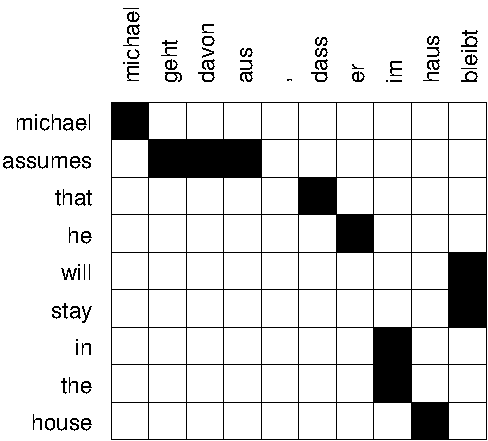
\includegraphics[scale=1.5]{michael-alignment.pdf}
\end{center}

%%%%%%%%%%%%%%%%%%%%%%%%%%%%%%%%%%%%%%%%%%%%%%%%%%%%%%%%%%%%%%%%%%%%%%%%%%%%

\slide{Word Alignment?}
\vspace{10mm}
\begin{center}
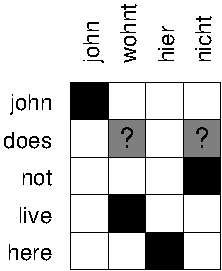
\includegraphics[scale=2]{does-not-alignment.pdf}\\[10mm]
Is the English word \example{does} aligned to\\ the German \example{wohnt} (verb) or \example{nicht} (negation) or neither?
\end{center}

%%%%%%%%%%%%%%%%%%%%%%%%%%%%%%%%%%%%%%%%%%%%%%%%%%%%%%%%%%%%%%%%%%%%%%%%%%%%

\slide{Word Alignment?}
\vspace{10mm}
\begin{center}
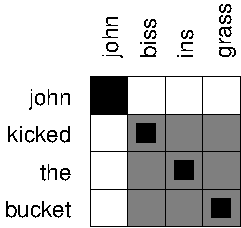
\includegraphics[scale=2]{kicked-the-bucket-alignment.pdf}\\[10mm]
How do the idioms \example{kicked the bucket} and \example{biss ins grass} match up?\\ Outside this exceptional context, \example{bucket} is never a good translation for \example{grass}
\end{center}

%%%%%%%%%%%%%%%%%%%%%%%%%%%%%%%%%%%%%%%%%%%%%%%%%%%%%%%%%%%%%%%%%%%%%%%%%%%%

\slide{Measuring Word Alignment Quality}
\vspace{10mm}
\begin{itemize}
\item Manually align corpus with {\em sure} (\maths{$S$}) and {\em possible} (\maths{$P$}) alignment points (\maths{$S \subseteq P$})
\item Common metric for evaluation word alignments: Alignment Error Rate (AER)
\maths{\begin{equation*}
\mbox{AER}(S,P;A) =  \frac{|A \cap S| + {|A \cap P|}}{|A|+|S|}
\end{equation*}}
\item AER = 0: alignment \maths{$A$} matches all sure, any possible alignment points
\item However: different applications require different precision/recall trade-offs
\end{itemize}

%%%%%%%%%%%%%%%%%%%%%%%%%%%%%%%%%%%%%%%%%%%%%%%%%%%%%%%%%%%%%%%%%%%%%%%%%%%%

\slide{Word Alignment with IBM Models}
\vspace{20mm}
\begin{itemize}
\item IBM Models create a {\bf many-to-one} mapping
{\begin{itemize}\itemsep 3mm
\item words are aligned using an alignment function
\item a function may return the same value for different input
\item[]  (one-to-many mapping)
\item a function can not return multiple values for one input
\item[]  (no many-to-one mapping)
\end{itemize} }
\item  Real word alignments have {\bf many-to-many} mappings
\end{itemize}



%%%%%%%%%%%%%%%%%%%%%%%%%%%%%%%%%%%%%%%%%%%%%%%%%%%%%%%%%%%%%%%%%%%%%%%%%%%%

\slide{Symmetrizing Word Alignments}
\vspace{-5mm}
\begin{center} 
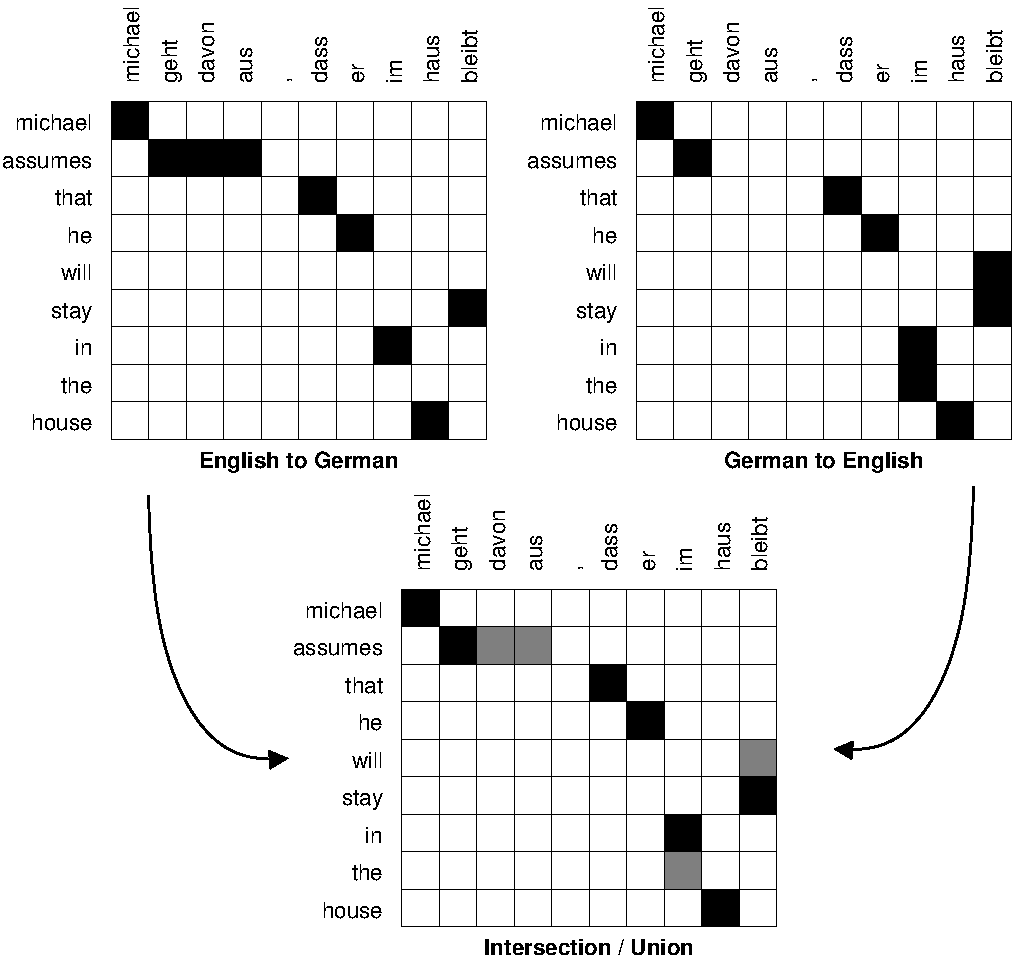
\includegraphics[scale=0.75]{michael-bidirectional.pdf}
\end{center}\vspace{-5mm}
\begin{itemize} \itemsep -5mm
\item Intersection of GIZA++ bidirectional alignments
\item Grow additional alignment points [Och~and~Ney,~CompLing2003]
\end{itemize}


%%%%%%%%%%%%%%%%%%%%%%%%%%%%%%%%%%%%%%%%%%%%%%%%%%%%%%%%%%%%%%%%%%%%%%%%%%%%
 
\slide{Growing heuristic}
\vspace{3mm}
{\footnotesize {\bf grow-diag-final}(e2f,f2e)
\begin{algorithmic}[1]
\STATE neighboring = $\{$(-1,0),(0,-1),(1,0),(0,1),(-1,-1),(-1,1),(1,-1),(1,1)$\}$
\STATE alignment $A$ = intersect(e2f,f2e); grow-diag(); final(e2f); final(f2e);
\end{algorithmic}
{\bf grow-diag}()
\begin{algorithmic}[1]
\WHILE{new points added}
\FORALL{English word $e \in [1 ... e_n]$, foreign word $f \in [1 ... f_n]$, $(e,f) \in A$}
      \FORALL{neighboring alignment points ($e_\text{new}$, $f_\text{new}$)}
         \IF{($e_\text{new}$ unaligned {\sc or} $f_\text{new}$ unaligned) {\sc and} ($e_\text{new},f_\text{new}) \in \text{union(e2f,f2e)}$}
           \STATE add ($e_\text{new},f_\text{new}$) to $A$
        \ENDIF
       \ENDFOR  
  \ENDFOR  
\ENDWHILE
\end{algorithmic}
{\bf final}()
\begin{algorithmic}[1]
\FORALL{English word $e_\text{new} \in [1 ... e_n]$, foreign word $f _\text{new}\in [1 ... f_n]$}
     \IF{($e_\text{new}$ unaligned {\sc or} $f_\text{new}$ unaligned) {\sc and} ($e_\text{new},f_\text{new}) \in \text{union(e2f,f2e)}$}
       \STATE add ($e_\text{new},f_\text{new}$) to $A$
     \ENDIF
\ENDFOR  
\end{algorithmic}
}

%%%%%%%%%%%%%%%%%%%%%%%%%%%%%%%%%%%%%%%%%%%%%%%%%%%%%%%%%%%%%%%%%%%%%%%%%%%%
 
\slide{More Recent Work on Symmetrization}
\vspace{15mm}
\begin{itemize}
\item Symmetrize after each iteration of IBM Models [Matusov et al., 2004]
\begin{itemize}
\item run one iteration of E-step for each direction
\item symmetrize the two directions
\item count collection (M-step)
\end{itemize}
\vspace{5mm}
\item Use of posterior probabilities in symmetrization 
\begin{itemize}
\item generate n-best alignments for each direction
\item calculate how often an alignment point occurs in these alignments
\item use this posterior probability during symmetrization
\end{itemize}
\end{itemize}

%%%%%%%%%%%%%%%%%%%%%%%%%%%%%%%%%%%%%%%%%%%%%%%%%%%%%%%%%%%%%%%%%%%%%%%%%%%%
 
\slide{Link Deletion / Addition Models}
\vspace{15mm}
\begin{itemize}
\item Link deletion [Fossum et al., 2008]
\begin{itemize}
\item start with union of IBM Model alignment points
\item delete one alignment point at a time
\item uses a neural network classifiers that also considers aspects such as how useful the alignment is for learning translation rules
\end{itemize}
\vspace{5mm}
\item Link addition [Ren et al., 2007] [Ma et al., 2008]
\begin{itemize}
\item possibly start with a skeleton of highly likely alignment points
\item add one alignment point at a time
\end{itemize}
\end{itemize}

%%%%%%%%%%%%%%%%%%%%%%%%%%%%%%%%%%%%%%%%%%%%%%%%%%%%%%%%%%%%%%%%%%%%%%%%%%%%
 
\slide{Discriminative Training Methods}
\vspace{10mm}
\begin{itemize}
\item Given some annotated training data, supervised learning methods are possible
\item Structured prediction
\begin{itemize}
\item not just a classification problem
\item solution structure has to be constructed in steps
\end{itemize}
\item Many approaches: maximum entropy, neural networks, support vector machines, conditional random fields, MIRA, ...
\item Small labeled corpus may be used for parameter tuning of unsupervised aligner [Fraser and Marcu, 2007]
\end{itemize}

%%%%%%%%%%%%%%%%%%%%%%%%%%%%%%%%%%%%%%%%%%%%%%%%%%%%%%%%%%%%%%%%%%%%%%%%%%%%
 
\slide{Better Generative Models}
\vspace{10mm}
\begin{itemize}
\item Aligning phrases
\begin{itemize}
\item joint model [Marcu and Wong, 2002]
\item problem: EM algorithm likes really long phrases
\end{itemize}
\vspace{10mm}
\item Fraser's LEAF
\begin{itemize}
\item decomposes word alignment into many steps
\item similar in spirit to IBM Models
\item includes step for grouping into phrase
\end{itemize}
\end{itemize}


%%%%%%%%%%%%%%%%%%%%%%%%%%%%%%%%%%%%%%%%%%%%%%%%%%%%%%%%%%%%%%%%%%%%%%%%%%%%

\slide{Summary}
\begin{itemize} \itemsep -1mm
\item Lexical translation
\item Alignment
\item Expectation Maximization (EM) Algorithm
\item Noisy Channel Model
\item IBM Models 1--5
\begin{itemize}
\item IBM Model 1: lexical translation
\item IBM Model 2: alignment model
\item IBM Model 3: fertility
\item IBM Model 4: relative alignment model
\item IBM Model 5: deficiency
\end{itemize}
\item Word Alignment
\end{itemize}
\end{document}
